% This work is made available under the terms of the
% Creative Commons Attribution-ShareAlike 4.0 license,
% http://creativecommons.org/licenses/by-sa/4.0/.

\documentclass[a4paper]{book}

\usepackage{wrapfig}
\usepackage{graphicx}
\usepackage{hyperref}
\usepackage{multirow}
\usepackage{scalefnt}
\usepackage{tikz}

% watermark -- for draft stage
%\usepackage[firstpage]{draftwatermark}
%\SetWatermarkLightness{0.9}
%\SetWatermarkScale{5}

% Copyright (c) 2009 by the University of Waikato, Hamilton, NZ. 
% This work is made available under the terms of the 
% Creative Commons Attribution-ShareAlike 4.0 license,
% http://creativecommons.org/licenses/by-sa/4.0/.
%
% Version: $Revision: 13214 $

\newenvironment{tight_itemize}{
\begin{itemize}
  \setlength{\itemsep}{1pt}
  \setlength{\parskip}{0pt}
  \setlength{\parsep}{0pt}}{\end{itemize}
}

\newenvironment{tight_enumerate}{
\begin{enumerate}
  \setlength{\itemsep}{1pt}
  \setlength{\parskip}{0pt}
  \setlength{\parsep}{0pt}}{\end{enumerate}
}

% if you just need a simple heading
% Usage:
%   \heading{the text of the heading}
\newcommand{\heading}[1]{
  \vspace{0.3cm} \noindent \textbf{#1} \newline
}

\newcommand{\icon}[1]{\tikz[baseline=-3pt]\node[inner sep=0pt,outer sep=0pt]{\includegraphics[height=1.1em]{#1}};}


\title{
  \textbf{ADAMS} \\
  {\Large \textbf{A}dvanced \textbf{D}ata mining \textbf{A}nd \textbf{M}achine
  learning \textbf{S}ystem} \\
  {\Large Module: adams-ufdl-image} \\
  \vspace{1cm}
  
\includegraphics[width=2cm]{images/ufdl-image-module.png} \\
}
\author{
  Peter Reutemann
}

\setcounter{secnumdepth}{3}
\setcounter{tocdepth}{3}

\begin{document}

\begin{titlepage}
\maketitle

\thispagestyle{empty}
\center
\begin{table}[b]
	\begin{tabular}{c l l}
		\parbox[c][2cm]{2cm}{\copyright 2019-2020} &
		\parbox[c][2cm]{5cm}{
\includegraphics[width=5cm]{images/coat_of_arms.pdf}} \\
	\end{tabular}
	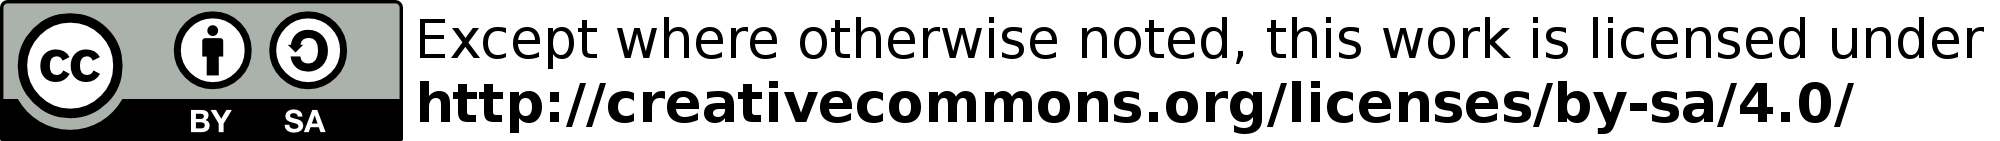
\includegraphics[width=12cm]{images/cc.png} \\
\end{table}

\end{titlepage}

\tableofcontents
%\listoffigures
%\listoftables

%%%%%%%%%%%%%%%%%%%%%%%%%%%%%%%%%%%
\chapter{UFDL}
UFDL, or user-friendly deep-learning, enables users with little or no deep-learning
expertise to maintain datasets for deep-learning tasks such as image classification
and object detection and also build deep-learnings models using these.

This ADAMS module focuses on image processing tasks.

%%%%%%%%%%%%%%%%%%%%%%%%%%%%%%%%%%%
\chapter{Flow}

In addition to the core UFDL components, you also have the following ones available.
These are used in the management flow \textit{adams-ufdl-image-manage\_image\_classification\_datasets.flow},
which can be used for administrating image classification datasets.

The following conversions are available:
\begin{tight_itemize}
  \item \textit{ReportToUFDLAnnotations} -- converts an ADAMS report to UFDL annotations
  \item \textit{UFDLAnnotationsToReport} -- converts UFDL annotations to an ADAMS report
  \item \textit{UFDLExtractImageNameFromFile} -- converts a file name into an image name used in datasets
  \item \textit{UFDLImageClassificationDatasetFilesToSpreadSheet} -- outputs all the files in an image classification dataset as spreadsheet
  \item \textit{UFDLImageClassificationDatasetToListItem} -- converts a UFDL ImageClassificationDataset to a list item string.
  \item \textit{UFDLImageClassificationDatasetToSpreadSheet} -- turns an image classification dataset into a spreadsheet
  \item \textit{UFDLObjectDetectionDatasetFilesToSpreadSheet} -- outputs all the files in an object detection dataset as spreadsheet
  \item \textit{UFDLObjectDetectionDatasetToListItem} -- converts a UFDL ObjectDetectionDataset to a list item string.
  \item \textit{UFDLObjectDetectionDatasetToSpreadSheet} -- turns an object detection dataset into a spreadsheet
\end{tight_itemize}

\section{Actions}
The following sink actions can be used:
\begin{tight_itemize}
  \item \textit{DownloadObjectDetectionDataset} -- downloads an object detection dataset
  \item \textit{DownloadImageClassificationDataset} -- downloads an image classification dataset
\end{tight_itemize}
The following source actions can be used:
\begin{tight_itemize}
  \item \textit{CreateImageClassificationDatasets} -- creates an image classification dataset
  \item \textit{CreateObjectDetectionDatasets} -- creates an object detection dataset
  \item \textit{ListImageClassificationDatasets} -- lists image classification datasets
  \item \textit{ListObjectDetectionDatasets} -- lists object detection datasets
\end{tight_itemize}
The following transformer actions can be used:
\begin{tight_itemize}
  \item \textit{AddImageClassificationCategoriesForFile} -- adds categories to images of an image classification dataset
  \item \textit{AddImageClassificationFile} -- adds images to an image classification dataset
  \item \textit{AddObjectDetectionFile} -- adds an image (and its optional annnotations) to an object detection dataset
  \item \textit{CopyImageClassificationDataset} -- copies the image classification dataset (new version or name)
  \item \textit{CopyObjectDetectionDataset} -- copies the object detection dataset (new version or name)
  \item \textit{DeleteImageClassificationCategoriesForFile} -- removes categories from images of an image classification dataset
  \item \textit{DeleteImageClassificationDataset} -- removes the specified image classification dataset
  \item \textit{DeleteImageClassificationFile} -- removes the specified image from an image classification dataset
  \item \textit{DeleteObjectDetectionDataset} -- removes the specified object detection dataset
  \item \textit{DeleteObjectDetectionFile} -- removes the specified image from an object detection dataset
  \item \textit{GetImageClassificationCategories} -- retrieves the map of image/categories for a dataset
  \item \textit{GetImageClassificationCategoriesForImage} -- retrieves the categories of an image from a dataset
  \item \textit{GetImageClassificationFile} -- retrieves a file from an image classification dataset via its name
  \item \textit{GetImageClassificationMetadata} -- retrieves the metadata for an image classification dataset
  \item \textit{GetImageClassificationMetadataForImage} -- retrieves the metadata for an image of an image classification dataset via its name
  \item \textit{GetObjectDetectionFile} -- retrieves a file from an object detection dataset via its name
  \item \textit{GetObjectDetectionLabels} -- retrieves the labels present in an object detection dataset
  \item \textit{GetObjectDetectionMetadata} -- retrieves the metadata for an object detection dataset
  \item \textit{GetObjectDetectionMetadataForImage} -- retrieves the metadata for an image of an object detection dataset via its name
  \item \textit{GetObjectDetectionAnnotations} -- obtains all the annotations from an object detection dataset
  \item \textit{GetObjectDetectionAnnotationsForImage} -- obtains the annotations of an image from an object detection dataset
  \item \textit{ListImageClassificationFiles} -- lists all the images in an image classification dataset
  \item \textit{ListObjectDetectionFiles} -- lists all the images in an object detection dataset
  \item \textit{LoadImageClassificationDataset} -- loads an image classification dataset (via PK)
  \item \textit{LoadObjectDetectionDataset} -- loads an object detection dataset (via PK)
  \item \textit{MergeImageClassificationDatasets} -- for merging two image classification datasets.
  \item \textit{MergeObjectDetectionDatasets} -- for merging two object detection datasets.
  \item \textit{ReinstateImageClassificationDataset} -- reinstates ("undeletes") an image classification dataset.
  \item \textit{ReinstateObjectDetectionDataset} -- reinstates ("undeletes") an object detection dataset.
  \item \textit{SetImageClassificationMetadataForImage} -- sets the metadata of an image in an object detection dataset
  \item \textit{SetObjectDetectionAnnotationsForImage} -- sets the annotations of an image in an object detection dataset
  \item \textit{SetObjectDetectionMetadataForImage} -- sets the metadata of an image in an object detection dataset
  \item \textit{UpdateImageClassificationDataset} -- updates the properties of an image classification dataset
  \item \textit{UpdateObjectDetectionDataset} -- updates the properties of an object detection dataset
\end{tight_itemize}

\section{EnterManyValues extensions}
The following extensions of value definitions used by the \textit{EnterManyValues}
source make it easier for users to select PKs:
\begin{tight_itemize}
  \item \textit{UFDLImageClassificationDatasetChooser} -- for selecting one or more image classification datasets
  \item \textit{UFDLImageClassificationDatasetList} -- for selecting an image classification dataset
  \item \textit{UFDLObjectDetectionDatasetChooser} -- for selecting one or more object detection datasets
  \item \textit{UFDLObjectDetectionDatasetList} -- for selecting an object detection dataset
\end{tight_itemize}

%%%%%%%%%%%%%%%%%%%%%%%%%%%%%%%%%%%
% This work is made available under the terms of the 
% Creative Commons Attribution-ShareAlike 4.0 license,
% http://creativecommons.org/licenses/by-sa/4.0/.
%
% Version: $Revision: 13411 $

\begin{thebibliography}{999}
	% to make the bibliography appear in the TOC
	\addcontentsline{toc}{chapter}{Bibliography}

    % references
	\bibitem{adams}
		\textit{ADAMS} -- Advanced Data mining and Machine learning System \\
		\url{https://adams.cms.waikato.ac.nz/}{}

\end{thebibliography}


\end{document}
